\documentclass{article}
\usepackage{iclr2026_conference,times}

\usepackage[utf8]{inputenc}
\usepackage[T1]{fontenc}
\usepackage{hyperref}
\usepackage{url}
\usepackage{booktabs}
\usepackage{nicefrac}
\usepackage{microtype}
\usepackage{xcolor}
\usepackage{graphicx}
\usepackage{subcaption}
\usepackage{multirow}
\usepackage{array}
\usepackage{amsmath,amssymb,amsfonts,amsthm,mathtools}
\usepackage[capitalize,noabbrev]{cleveref}
\usepackage[section]{placeins}

\input{math_commands}

\newcommand{\pending}{\textit{pending}}
\newcommand{\gelu}{\textsc{Gelu}}
\newcommand{\patchtst}{PatchTST}
\newcommand{\itransformer}{iTransformer}

\title{Activations Are Not Defaults:\\
Dataset- and Regime-Dependent Nonlinearity Selection for Long-Horizon Forecasting}

\author{Anonymous Authors}

\begin{document}

\maketitle

\begin{abstract}
Activation functions in time-series forecasting models are usually treated as implementation defaults, while most methodological work focuses on architectures, attention mechanisms, input windows, and losses. We challenge this convention by studying activation-only interventions under fixed forecasting protocols. In a completed Informer full-grid study covering 36 dataset-horizon cells, nine activation configurations, and three seeds per configuration, non-\gelu{} activations are best in 34 of 36 cells; bounded and tanh-family activations achieve the strongest average ranks. These results show that activation choice is a first-order design variable even when attention, width, depth, optimizer, and training schedule are held fixed. The same grid also rejects a universal-activation story: Solar3 remains \gelu{}-best at both horizons, output tanh is highly beneficial in selected long-horizon ETT/ETTm cells but weak on average, and decoder-only tanh wins no cell. Transfer stress tests sharpen this boundary. In \patchtst{}, non-\gelu{} activations are best in 5 of 12 tested cells, but \gelu{} remains best in 7 cells, and output tanh loses all 54 paired comparisons against matched linear heads. In a one-seed \itransformer{} pilot, \gelu{} remains best in 5 of 6 ETTh2/ETTm2 cells, with only a narrow \texttt{tanh\_sin001} win on ETTm2/96. We therefore frame activation selection as a conditional and architecture-dependent problem over activation family, placement, dataset, horizon, and input-window regime. The remaining submission gap is prospective factor-conditioned selection of activation regime and placement.
\end{abstract}

\section{Introduction}

Long-horizon forecasting papers often frame progress as architectural: more efficient attention, patching, decomposition, channel handling, or improved temporal embeddings. In contrast, the nonlinearity inside feed-forward blocks is commonly inherited from the reference implementation. This is a strong implicit assumption. A forecasting model's activation function controls saturation, sign preservation, gradient scale, and sensitivity to large input excursions. These properties are directly relevant to time-series data, where volatility, jumps, trends, reversals, and heavy tails vary across datasets and horizons.

This paper studies a deliberately narrow question: if the forecasting architecture, optimizer, data split, horizon-specific window, and training schedule are fixed, can changing only the activation function and its placement materially improve performance? Our completed answer for Informer is yes. Across ETTh1, ETTh2, ETTm1, ETTm2, and eight Solar sites, we evaluate 36 dataset-horizon cells, nine activation configurations, and three seeds per configuration. Non-\gelu{} activations are best in 34 of 36 cells. The best average ranks belong to tanh-family and bounded activations: \texttt{tanh\_sin001\_all}, \texttt{tanh\_all}, and \texttt{softsign\_all}. These gains are not confined to one dataset: all 20 ETT/ETTm cells and 14 of 16 Solar cells prefer a non-\gelu{} activation.

At the same time, our evidence argues against a universal activation. The best configuration varies across dataset and horizon. Output tanh wins several long-horizon ETT/ETTm cells but is weak globally. Encoder-side tanh is strongest in selected Solar96 cells. Decoder-only tanh never wins. Solar3 remains \gelu{}-best at both tested horizons. The scientific story is therefore not that we discovered a single replacement for \gelu{}, but that activation choice is conditional.

The natural next question is whether this conditionality can be predicted from the data itself. We explore this using factor-bin diagnostics inspired by financial regime analysis. Input windows are summarized by volatility, realized volatility, jump intensity, trend consistency, max absolute change, tail ratio, reversal rate, mean reversion strength, and related factors. The goal is to determine whether these factors can predict both the activation regime and its placement, enabling low-cost activation selection without modifying the forecasting architecture.

The present evidence is not yet sufficient to claim a deployed zero-shot selector. Summary-level factor bins reveal regime dependence across the full matrix, but the stricter leave-one-seed-out oracle is positive only in Solar1/96. Therefore, this draft treats factor bins as a mechanism and selection-design tool until a prospective router experiment is completed. The \patchtst{} and \itransformer{} probes are now filled as architecture-transfer stress tests: they show activation sensitivity in selected cells, but they do not support broad portability of the Informer ranking.

\paragraph{Contributions.}
This draft organizes the paper around six contributions. First, we isolate activation family and placement in Informer while holding attention, width, depth, optimizer, data splits, and training protocol fixed. Second, we provide a complete three-seed Informer matrix of 972 seed-runs across 36 dataset-horizon cells and nine activation configurations. Third, we show that bounded and tanh-family activations are the strongest static candidates, while the complete grid rejects a universal winner. Fourth, we disentangle placement effects by separating full-hidden replacement, encoder-only tanh, decoder-only tanh, and hidden-plus-output tanh. Fifth, we introduce factor-bin diagnostics and specify the prospective experiment required to test whether input-window factors can select activation regime and placement. Sixth, we run \patchtst{} and \itransformer{} transfer stress tests showing that activation sensitivity can persist outside Informer, but the best family and placement are architecture-dependent.

% Generated by figures/gen_phase4_paper_assets.py
\begin{figure*}[t]
    \centering
    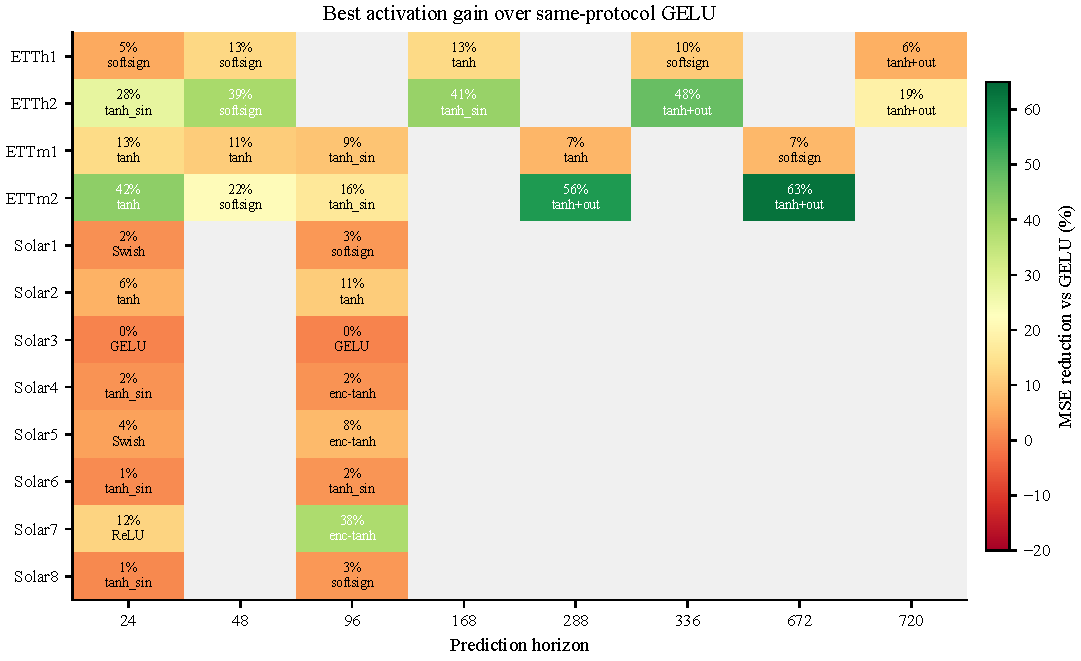
\includegraphics[width=\textwidth]{figures/fig_phase4_best_gain_heatmap.pdf}
    \caption{Best activation gain over the same-protocol GELU row in each completed dataset-horizon cell. The full grid covers 36 dataset-horizon cells, nine activation configurations, and three seeds. Most cells prefer a non-GELU activation, but Solar3 remains GELU-best at both horizons.}
    \label{fig:phase4_best_gain_heatmap}
\end{figure*}

\begin{figure}[t]
    \centering
    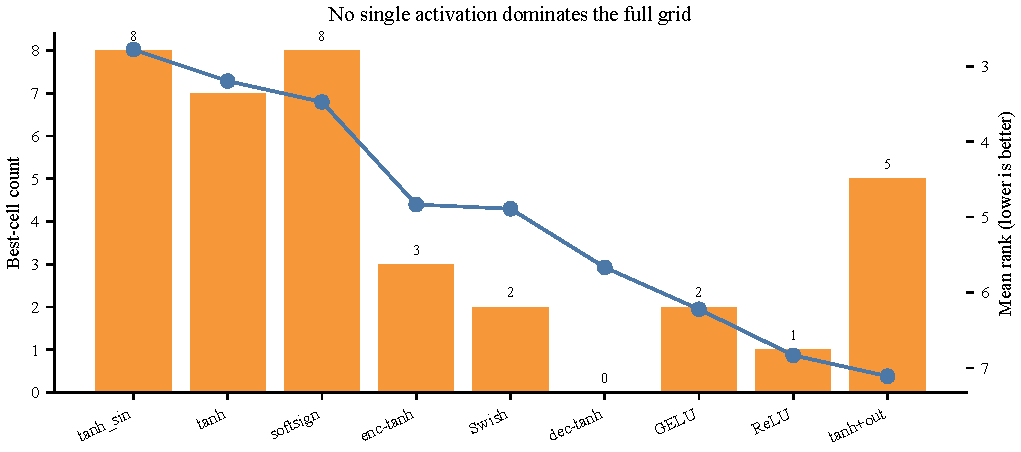
\includegraphics[width=\linewidth]{figures/fig_phase4_static_ranking.pdf}
    \caption{Static activation ranking across the full Phase-4 grid. Bounded and tanh-family activations rank best on average, but the best-cell counts are spread across several configurations, arguing against a universal replacement activation.}
    \label{fig:phase4_static_ranking}
\end{figure}


\section{Related Work}

\paragraph{Transformer forecasting architectures.}
Informer \citep{zhou2021informer} adapts transformer sequence modeling \citep{vaswani2017attention} to long-sequence forecasting through ProbSparse attention and an encoder-decoder design. \patchtst{} \citep{nie2023patchtst} represents a different architectural family, using patch-level temporal tokens and channel-independent modeling. \itransformer{} \citep{liu2023itransformer} inverts the tokenization view by treating variates as tokens. Our completed evidence uses Informer as the controlled full-grid substrate and uses \patchtst{} and \itransformer{} as architecture-transfer stress tests.

\paragraph{Activation functions.}
ReLU \citep{nair2010relu} and \gelu{} \citep{hendrycks2016gelu} are common defaults in deep networks. Bounded activations such as tanh and softsign are older, but they impose qualitatively different behavior: they preserve sign while constraining magnitude. Our results show that these properties can matter in forecasting even when no architectural component changes.

\paragraph{Oscillatory and Fourier-style nonlinearities.}
Periodic activations and Fourier features have been studied for representing high-frequency functions \citep{sitzmann2020siren,tancik2020fourier}. Our use of oscillatory activations is more conservative: we test a small tanh-centered sinusoidal perturbation inside a forecasting transformer. The current result is that this perturbation is a strong static candidate, not that oscillation should be selected in every volatile regime.

\paragraph{Regime-conditioned analysis.}
Forecasting errors are often regime-dependent. We therefore bind test windows to input factors such as volatility, jumps, trend consistency, and reversals. This paper distinguishes two levels of evidence: post hoc factor-bin diagnostics, which reveal where activations differ, and prospective factor-conditioned routing, which must choose activation and placement before seeing test errors.

\section{Hypotheses}

\paragraph{H1: Activation functions are first-order design variables.}
Changing only activation family or placement, while holding architecture and protocol fixed, can materially change forecasting performance. This hypothesis is supported in Informer by 972 completed seed-runs and 34/36 non-\gelu{} best cells.

\paragraph{H2: Bounded and tanh-family activations are strong static candidates.}
Bounded/sign-preserving nonlinearities and small tanh-centered oscillatory perturbations can outperform \gelu{}-style defaults in many forecasting regimes. This hypothesis is supported as a static recommendation, but not as a universal winner.

\paragraph{H3: Oscillatory perturbations help in some regimes, but are not universally tied to volatility.}
\texttt{tanh\_sin001\_all} has the best mean rank in the Informer grid, but the current factor-bin evidence does not justify a direct rule such as ``high volatility implies oscillatory activation.'' A prospective factor-router experiment is required.

\paragraph{H4: Placement matters and can reverse the effect of the same activation.}
Full-hidden replacement, encoder-only tanh, decoder-only tanh, and output tanh have different empirical profiles. This hypothesis is supported: full-hidden placement wins 28 cells, hidden-plus-output tanh wins five, encoder-only tanh wins three, and decoder-only tanh wins none.

\paragraph{H5: Input-window factors can predict activation regime and placement.}
This is the central open hypothesis. Current factor-bin diagnostics show regime dependence, but they do not yet prove predictive selection. The final claim requires a rule that uses only input-window factors and is evaluated on held-out seeds, sites, horizons, or future windows.

\section{Method}

\subsection{Activation-only interventions}

Let \(X_{t-L+1:t}\in\mathbb{R}^{L\times C}\) denote an input window and let the model predict \(Y_{t+1:t+H}\). We define an activation-only intervention as changing the nonlinearity used inside the forecasting model while keeping the architecture, attention, width, depth, optimizer, training schedule, data split, and horizon-specific windows fixed. In Informer, the intervention is applied to encoder and decoder feed-forward blocks, with an optional output activation used only for explicit placement tests.

\begin{table}[!htbp]
\centering
\caption{Activation configurations used in the completed Informer grid.}
\label{tab:activation_configs_draft}
\resizebox{\textwidth}{!}{%
\begin{tabular}{lllll}
\toprule
Config & Encoder FFN & Decoder FFN & Output & Purpose \\
\midrule
\texttt{gelu\_all} & GELU & GELU & Linear & Same-protocol baseline \\
\texttt{relu\_all} & ReLU & ReLU & Linear & Monotone non-bounded control \\
\texttt{swish\_all} & Swish & Swish & Linear & Smooth non-bounded control \\
\texttt{tanh\_all} & tanh & tanh & Linear & Bounded sign-preserving candidate \\
\texttt{softsign\_all} & softsign & softsign & Linear & Bounded sign-preserving candidate \\
\texttt{tanh\_sin001\_all} & tanh \(+0.01\sin\) & tanh \(+0.01\sin\) & Linear & Small oscillatory perturbation \\
\texttt{enc\_tanh\_dec\_gelu} & tanh & GELU & Linear & Encoder-placement test \\
\texttt{enc\_gelu\_dec\_tanh} & GELU & tanh & Linear & Decoder-placement test \\
\texttt{tanh\_all\_outtanh} & tanh & tanh & tanh & Hidden plus output-bounding test \\
\bottomrule
\end{tabular}%
}
\end{table}

\subsection{Factor-bin diagnostics}

For each input window, we compute regime factors: volatility, realized volatility, volatility shock, max absolute change, jump intensity, tail ratio, trend consistency, reversal rate, mean reversion strength, range, skewness, kurtosis, and downside/upside volatility. We use these factors in two ways. Summary-level factor bins group dataset-horizon cells and cover the full completed matrix; they are diagnostic but not deployable. Sample-level oracles use saved prediction arrays to estimate the benefit of choosing different activations in different factor bins. Same-split oracles are upper bounds. Leave-one-seed-out oracles provide weak generalization evidence.

\subsection{Prospective factor router}

The missing mechanism experiment is a prospective router. The router can use only input-window factors and must select both activation regime and placement before evaluation. Its action space should remain small enough to validate: \gelu{}, \texttt{tanh\_sin001\_all}, \texttt{tanh\_all}, \texttt{softsign\_all}, \texttt{enc\_tanh\_dec\_gelu}, and \texttt{tanh\_all\_outtanh}. It must be compared against \gelu{}, the best static activation, and the same-split oracle upper bound.

\begin{table}[!htbp]
\centering
\caption{Candidate prospective routers. Results are intentionally left pending in this hypothesis draft.}
\label{tab:router_forms}
\resizebox{\textwidth}{!}{%
\begin{tabular}{lll}
\toprule
Router & Description & Claim strength if successful \\
\midrule
Rule-based threshold & Hand-designed thresholds on volatility, jumps, and trend factors & Weak but interpretable \\
Cell-trained decision tree & Learn factor-to-activation rules on training cells & Moderate \\
Leave-dataset-out router & Train on all but one dataset/site, test on held-out site & Strong \\
Leave-horizon-out router & Train on some horizons, test on unseen horizon & Strong \\
Uncertainty-gated router & Choose best static activation unless confidence is high & Most practical \\
\bottomrule
\end{tabular}%
}
\end{table}

\section{Completed Informer Evidence}

\subsection{Full-grid coverage}

The completed Informer Phase-4 matrix contains 972 eligible seed-runs: 36 dataset-horizon cells, nine activation configurations, and three seeds per configuration. All 324 dataset-horizon-configuration cells have complete three-seed coverage under batch size 32 and six epochs.

\begin{table*}[t]
\centering
\caption{Phase-4 full-grid coverage. A main-table cell is eligible only when all three seeds are present under batch size 32 and six training epochs.}
\label{tab:phase4_coverage}
\resizebox{\textwidth}{!}{%
\begin{tabular}{lrrrr}
\toprule
Group & dataset-horizon cells & config cells & seed-runs & 3-seed config cells \\
\midrule
ETTh & 10 & 90 & 270/270 & 90/90 \\
ETTm & 10 & 90 & 270/270 & 90/90 \\
Solar & 16 & 144 & 432/432 & 144/144 \\
All & 36 & 324 & 972/972 & 324/324 \\
\bottomrule
\end{tabular}%
}
\end{table*}


\subsection{Activation-only changes beat GELU in most cells}

\Cref{fig:phase4_best_gain_heatmap} summarizes the main result. Non-\gelu{} activations are best in 34 of 36 cells. The only \gelu{}-best cases are Solar3 at horizons 24 and 96. ETT and ETTm cells show the largest gains: all 20 ETT/ETTm cells prefer non-\gelu{} activations, with mean best-cell MSE reductions of 22.1\% on ETTh and 24.7\% on ETTm. Solar gains are smaller and more site-specific: 14 of 16 Solar cells prefer non-\gelu{} activations.

\begin{table*}[t]
\centering
\caption{Static activation ranking across the 36 completed dataset-horizon cells. Rank is computed within each cell over the nine Phase-4 configurations.}
\label{tab:phase4_static_ranking}
\resizebox{\textwidth}{!}{%
\begin{tabular}{lrrrrr}
\toprule
Config & mean rank & best cells & top-3 cells & mean gain & positive cells \\
\midrule
tanh\_sin & 2.78 & 8 & 27 & +11.7\% & 83.3\% \\
tanh & 3.19 & 7 & 25 & +11.9\% & 80.6\% \\
softsign & 3.47 & 8 & 22 & +11.2\% & 80.6\% \\
enc-tanh & 4.83 & 3 & 11 & +5.1\% & 66.7\% \\
Swish & 4.89 & 2 & 5 & +3.6\% & 77.8\% \\
dec-tanh & 5.67 & 0 & 3 & +1.9\% & 66.7\% \\
GELU & 6.22 & 2 & 4 & +0.0\% & 0.0\% \\
ReLU & 6.83 & 1 & 4 & -2.3\% & 36.1\% \\
tanh+out & 7.11 & 5 & 7 & -36.3\% & 25.0\% \\
\bottomrule
\end{tabular}%
}
\end{table*}


The static ranking shows that the strongest average configurations are \texttt{tanh\_sin001\_all}, \texttt{tanh\_all}, and \texttt{softsign\_all}. This supports bounded/tanh-family activations as strong static candidates, but the best-cell wins are distributed across multiple configurations. This is the empirical reason to frame the result as conditional selection rather than universal replacement.

\subsection{Placement is conditional}

Placement effects are substantial. Full-hidden replacement is the most stable default, winning 28 of 36 cells. Hidden-plus-output tanh wins five long-horizon ETT/ETTm cells: ETTh1/720, ETTh2/336, ETTh2/720, ETTm2/288, and ETTm2/672. Encoder-only tanh wins Solar4/96, Solar5/96, and Solar7/96. Decoder-only tanh wins no cell. These results rule out the interpretation that all gains come from output clipping or any single insertion point.

\subsection{Factor-bin diagnostics reveal dependence but not routing}

Summary-level factor bins cover all 36 dataset-horizon cells and produce 783 factor-bin rows. They reveal many factor-conditioned contrasts, which indicates that activation differences vary with regime summaries. The stricter sample-level leave-one-seed-out oracle is much weaker: among 84 oracle rows, only seven are positive, all on Solar1/96.

\begin{table*}[t]
\centering
\caption{Top positive leave-one-seed-out factor-oracle diagnostics among array-ready Phase-4 cells. These are diagnostic upper bounds for regime sensitivity, not deployed activation-routing results.}
\label{tab:phase4_loso_oracle}
\resizebox{\textwidth}{!}{%
\begin{tabular}{lllccc}
\toprule
Dataset & H & factor & LOSO oracle MSE & best static MSE & gain \\
\midrule
Solar1 & 96 & max\_abs\_change & 0.174 & 0.178 & +2.0\% \\
Solar1 & 96 & volatility & 0.175 & 0.178 & +1.4\% \\
Solar1 & 96 & volatility\_shock & 0.175 & 0.178 & +1.3\% \\
Solar1 & 96 & trend\_consistency & 0.177 & 0.178 & +0.4\% \\
Solar1 & 96 & max\_drawdown & 0.177 & 0.178 & +0.2\% \\
Solar1 & 96 & max\_drawup & 0.177 & 0.178 & +0.2\% \\
Solar1 & 96 & range & 0.177 & 0.178 & +0.2\% \\
\bottomrule
\end{tabular}%
}
\end{table*}


Thus, factor bins are useful for mechanism diagnosis and experiment design, but the current evidence does not support a deployed router. The router must be validated prospectively.

\section{Completed Experiment A: PatchTST Transfer}

\subsection{Goal}

This experiment tests whether activation sensitivity transfers from Informer to \patchtst{}. The result is partial: activation choice still matters in selected cells, but the Informer static ranking and output-tanh placement do not directly transfer.

\subsection{Transfer results}

\begin{table}[t]
\centering
\caption{PatchTST activation-transfer stress test. The Informer activation effect transfers only partially: non-GELU activations win selected ETTh2/Solar cells, while GELU remains best in 7 of 12 tested cells.}
\label{tab:patchtst_transfer}
\begin{tabular}{llrrlr}
\toprule
Model & Dataset & Horizon & GELU MSE & Best config & Gain \\
\midrule
PatchTST & ETTh2 & 168 & 0.325880 & \texttt{gelu\_ffn\_linear} & 0.00\% \\
PatchTST & ETTh2 & 336 & 0.328450 & \texttt{gelu\_ffn\_linear} & 0.00\% \\
PatchTST & ETTh2 & 720 & 0.380881 & \texttt{softsign\_ffn\_linear} & 0.67\% \\
PatchTST & ETTm2 & 96 & 0.165589 & \texttt{gelu\_ffn\_linear} & 0.00\% \\
PatchTST & ETTm2 & 288 & 0.262739 & \texttt{gelu\_ffn\_linear} & 0.00\% \\
PatchTST & ETTm2 & 672 & 0.355232 & \texttt{gelu\_ffn\_linear} & 0.00\% \\
PatchTST & Solar2 & 24 & 0.065450 & \texttt{tanh\_sin001\_ffn\_linear} & 0.42\% \\
PatchTST & Solar2 & 96 & 0.099666 & \texttt{softsign\_ffn\_linear} & 1.12\% \\
PatchTST & Solar3 & 24 & 0.279035 & \texttt{gelu\_ffn\_linear} & 0.00\% \\
PatchTST & Solar3 & 96 & 0.446409 & \texttt{gelu\_ffn\_linear} & 0.00\% \\
PatchTST & Solar5 & 24 & 0.114792 & \texttt{tanh\_sin001\_ffn\_linear} & 1.33\% \\
PatchTST & Solar5 & 96 & 0.176366 & \texttt{softsign\_ffn\_linear} & 1.01\% \\
\bottomrule
\end{tabular}
\end{table}


\begin{table}[t]
\centering
\caption{PatchTST output-tanh placement test. Output tanh loses every paired seed-run comparison against the matching linear-head configuration, indicating that the Informer output-bounding signal does not transfer to PatchTST.}
\label{tab:patchtst_output_tanh}
\begin{tabular}{lrrr}
\toprule
Base activation & Paired seed-runs & Win rate & Mean gain vs. linear \\
\midrule
\texttt{tanh} & 18 & 0.0\% & -5.28\% \\
\texttt{tanh\_sin001} & 18 & 0.0\% & -5.31\% \\
\texttt{gelu} & 18 & 0.0\% & -5.44\% \\
\bottomrule
\end{tabular}
\end{table}


\paragraph{Interpretation.}
Non-\gelu{} activations win 5 of 12 \patchtst{} cells, concentrated in ETTh2/720 and Solar2/Solar5. \gelu{} remains best in 7 cells, including all tested ETTm2 horizons and both Solar3 horizons. Output tanh loses all 54 paired seed-run comparisons against matching linear-head configurations. The paper should therefore claim architecture-sensitive transfer: activation choice remains relevant outside Informer, but neither the Informer ranking nor output-bounding placement is portable as a default rule.

\section{Completed Experiment B: iTransformer Transfer}

\subsection{Goal}

This experiment asks whether the same FFN activation families transfer to \itransformer{}. It is intentionally smaller than the \patchtst{} study: one seed, two ETT datasets, three horizons, and no output-placement variants. It should therefore be read as a fast architecture-transfer probe rather than a final multi-seed claim.

\subsection{Transfer results}

\begin{table}[t]
\centering
\caption{iTransformer activation-transfer stress test. In this one-seed pilot, GELU remains best in 5 of 6 ETTh2/ETTm2 cells; the only non-GELU win is a narrow \texttt{tanh\_sin001} gain on ETTm2/96.}
\label{tab:itransformer_transfer}
\begin{tabular}{llrrlr}
\toprule
Model & Dataset & Horizon & GELU MSE & Best config & Gain \\
\midrule
iTransformer & ETTh2 & 96 & 0.301598 & \texttt{gelu\_ffn\_linear} & 0.00\% \\
iTransformer & ETTh2 & 336 & 0.422894 & \texttt{gelu\_ffn\_linear} & 0.00\% \\
iTransformer & ETTh2 & 720 & 0.428986 & \texttt{gelu\_ffn\_linear} & 0.00\% \\
iTransformer & ETTm2 & 96 & 0.184226 & \texttt{tanh\_sin001\_ffn\_linear} & 0.19\% \\
iTransformer & ETTm2 & 336 & 0.313418 & \texttt{gelu\_ffn\_linear} & 0.00\% \\
iTransformer & ETTm2 & 720 & 0.414092 & \texttt{gelu\_ffn\_linear} & 0.00\% \\
\bottomrule
\end{tabular}
\end{table}


\paragraph{Interpretation.}
\itransformer{} is a stricter negative/weak transfer test. \gelu{} remains best in 5 of 6 ETTh2/ETTm2 cells. The only non-\gelu{} win is ETTm2/96, where \texttt{tanh\_sin001\_ffn\_linear} improves MSE over \gelu{} by 0.19\%. This does not support direct migration of the Informer tanh-family ranking to \itransformer{}. Instead, together with the \patchtst{} result, it supports the narrower claim that activation effects are architecture-dependent and should be selected conditionally.

\section{Missing Experiment C: Factor-Conditioned Selection}

\subsection{Goal}

The second missing experiment tests whether input-window factors can prospectively predict activation regime and placement. This experiment determines whether the paper can claim a selection mechanism rather than only a diagnostic map.

\subsection{Validation matrix}

\begin{table}[!htbp]
\centering
\caption{Prospective factor-router validation matrix.}
\label{tab:router_validation_matrix}
\resizebox{\textwidth}{!}{%
\begin{tabular}{llll}
\toprule
Validation split & Train source & Test target & Required output \\
\midrule
Leave-one-seed-out & Two seeds in same cell & Held-out seed & Router MSE vs best static \\
Leave-one-Solar-site-out & Solar sites except one & Held-out Solar site & Generalization across sites \\
Leave-one-horizon-out & Some horizons & Unseen horizon & Horizon transfer \\
Future-window split & Earlier test windows & Later test windows & Time-forward robustness \\
Leave-family-out & ETT train, Solar test or inverse & Held-out family & Cross-family robustness \\
\bottomrule
\end{tabular}%
}
\end{table}

\begin{table}[!htbp]
\centering
\caption{Planned prospective factor-router result table.}
\label{tab:router_results_placeholder}
\resizebox{\textwidth}{!}{%
\begin{tabular}{llccccc}
\toprule
Split & Scope & GELU MSE & Best static MSE & Oracle MSE & Router MSE & Gain vs static \\
\midrule
Leave-one-seed-out & \pending & \pending & \pending & \pending & \pending & \pending \\
Leave-one-Solar-site-out & \pending & \pending & \pending & \pending & \pending & \pending \\
Leave-one-horizon-out & \pending & \pending & \pending & \pending & \pending & \pending \\
Future-window split & \pending & \pending & \pending & \pending & \pending & \pending \\
Leave-family-out & \pending & \pending & \pending & \pending & \pending & \pending \\
\bottomrule
\end{tabular}%
}
\end{table}

\begin{table}[!htbp]
\centering
\caption{Planned mechanism table for factor-to-placement rules.}
\label{tab:router_mechanism_placeholder}
\resizebox{\textwidth}{!}{%
\begin{tabular}{lllll}
\toprule
Factor condition & Selected activation & Selected placement & Held-out evidence & Use in final paper? \\
\midrule
High volatility + high max absolute change & \pending & \pending & \pending & \pending \\
High trend consistency & \pending & \pending & \pending & \pending \\
High jump intensity & \pending & \pending & \pending & \pending \\
High reversal rate & \pending & \pending & \pending & \pending \\
Low volatility + stable trend & \pending & \pending & \pending & \pending \\
\bottomrule
\end{tabular}%
}
\end{table}

\FloatBarrier

\paragraph{Success criteria.}
The router must beat \gelu{}. It should beat or match the best static activation on at least one held-out split. It should not collapse on counterexample cells such as Solar3. Its rules should be interpretable, because the claim is not merely that an oracle exists but that factors can guide activation and placement selection before evaluation.

\section{Discussion}

The completed Informer grid already supports a meaningful paper: activations are not harmless defaults in long-horizon forecasting. The completed \patchtst{} and \itransformer{} stress tests narrow the generality claim: activation sensitivity is not purely an Informer artifact, but the activation ranking and placement policy are architecture-dependent. Prospective factor routing remains the key missing experiment that determines whether factor bins can move from diagnosis to prediction.

This draft therefore uses a claim ladder. The safe claim is that activation choice is dataset- and horizon-sensitive in Informer. The cross-architecture claim is weaker but still useful: activation sensitivity remains visible in selected \patchtst{} and \itransformer{} cells, while the best activation family and placement are architecture-dependent. The strongest claim, only after router validation, is that activation regime and placement can be selected from data characteristics to improve forecasting without modifying the model architecture.

\section{Conclusion}

Our current evidence shows that activation-only interventions can substantially change Informer forecasting performance under fixed protocols. Non-\gelu{} activations win 34 of 36 dataset-horizon cells, and bounded/tanh-family activations are the best static candidates on average. Yet the same evidence rejects a universal activation: placement, dataset, horizon, regime, and architecture all matter. \patchtst{} confirms that transfer is partial and output tanh fails consistently; \itransformer{} further shows that \gelu{} can remain the strongest default in a different transformer variant. The final submission should therefore be built around conditional activation selection. The remaining work is sharply defined: test whether factor bins can prospectively select activation regime and placement.

\FloatBarrier

\bibliography{references}
\bibliographystyle{iclr2026_conference}

\newpage
\appendix

\section{Additional Informer Best-Cell Table}

\begin{table*}[t]
\centering
\caption{Best activation per dataset-horizon in the completed Phase-4 grid. Improvements are relative MSE reductions against the same-protocol GELU row with matched seeds; GELU-best cells have no relative-improvement entry.}
\label{tab:phase4_best_activation}
\resizebox{\textwidth}{!}{%
\begin{tabular}{llcccc}
\toprule
Dataset & H & best config & MSE & gain vs GELU & seed win rate \\
\midrule
ETTh1 & 24 & softsign & 0.532 $\pm$ 0.026 & +5.2\% & 66.7\% \\
ETTh1 & 48 & softsign & 0.646 $\pm$ 0.073 & +12.6\% & 100.0\% \\
ETTh1 & 168 & tanh & 0.912 $\pm$ 0.131 & +12.9\% & 66.7\% \\
ETTh1 & 336 & softsign & 1.219 $\pm$ 0.042 & +10.4\% & 100.0\% \\
ETTh1 & 720 & tanh+out & 1.328 $\pm$ 0.030 & +6.0\% & 100.0\% \\
ETTh2 & 24 & tanh\_sin & 0.516 $\pm$ 0.023 & +27.8\% & 100.0\% \\
ETTh2 & 48 & softsign & 1.606 $\pm$ 0.386 & +38.8\% & 100.0\% \\
ETTh2 & 168 & tanh\_sin & 2.963 $\pm$ 0.509 & +41.3\% & 100.0\% \\
ETTh2 & 336 & tanh+out & 2.054 $\pm$ 0.219 & +47.7\% & 100.0\% \\
ETTh2 & 720 & tanh+out & 3.298 $\pm$ 0.186 & +18.6\% & 100.0\% \\
ETTm1 & 24 & tanh & 0.314 $\pm$ 0.015 & +13.4\% & 100.0\% \\
ETTm1 & 48 & tanh & 0.453 $\pm$ 0.023 & +10.8\% & 100.0\% \\
ETTm1 & 96 & tanh\_sin & 0.559 $\pm$ 0.050 & +9.3\% & 100.0\% \\
ETTm1 & 288 & tanh & 0.802 $\pm$ 0.044 & +7.2\% & 66.7\% \\
ETTm1 & 672 & softsign & 0.922 $\pm$ 0.023 & +7.3\% & 66.7\% \\
ETTm2 & 24 & tanh & 0.685 $\pm$ 0.191 & +42.5\% & 100.0\% \\
ETTm2 & 48 & softsign & 0.309 $\pm$ 0.014 & +21.6\% & 100.0\% \\
ETTm2 & 96 & tanh\_sin & 1.335 $\pm$ 0.214 & +16.4\% & 100.0\% \\
ETTm2 & 288 & tanh+out & 2.355 $\pm$ 0.359 & +55.7\% & 100.0\% \\
ETTm2 & 672 & tanh+out & 2.851 $\pm$ 0.162 & +62.7\% & 100.0\% \\
Solar1 & 24 & Swish & 0.150 $\pm$ 0.000 & +1.7\% & 66.7\% \\
Solar1 & 96 & softsign & 0.224 $\pm$ 0.001 & +2.6\% & 100.0\% \\
Solar2 & 24 & tanh & 0.066 $\pm$ 0.003 & +6.4\% & 100.0\% \\
Solar2 & 96 & tanh & 0.108 $\pm$ 0.005 & +10.8\% & 100.0\% \\
Solar3 & 24 & GELU & 0.198 $\pm$ 0.009 & -- & -- \\
Solar3 & 96 & GELU & 0.349 $\pm$ 0.007 & -- & -- \\
Solar4 & 24 & tanh\_sin & 0.220 $\pm$ 0.003 & +1.9\% & 100.0\% \\
Solar4 & 96 & enc-tanh & 0.290 $\pm$ 0.005 & +1.9\% & 66.7\% \\
Solar5 & 24 & Swish & 0.109 $\pm$ 0.002 & +4.2\% & 100.0\% \\
Solar5 & 96 & enc-tanh & 0.180 $\pm$ 0.003 & +7.6\% & 100.0\% \\
Solar6 & 24 & tanh\_sin & 0.265 $\pm$ 0.002 & +1.1\% & 100.0\% \\
Solar6 & 96 & tanh\_sin & 0.358 $\pm$ 0.009 & +2.3\% & 100.0\% \\
Solar7 & 24 & ReLU & 3.281 $\pm$ 1.035 & +12.0\% & 66.7\% \\
Solar7 & 96 & enc-tanh & 4.970 $\pm$ 1.353 & +38.2\% & 100.0\% \\
Solar8 & 24 & tanh\_sin & 0.216 $\pm$ 0.003 & +0.8\% & 100.0\% \\
Solar8 & 96 & softsign & 0.306 $\pm$ 0.005 & +2.6\% & 100.0\% \\
\bottomrule
\end{tabular}%
}
\end{table*}


\section{Pending Experiment Summary}

\begin{table}[!htbp]
\centering
\caption{Final missing experiments before the strongest submission claim.}
\label{tab:pending_summary}
\resizebox{\textwidth}{!}{%
\begin{tabular}{llll}
\toprule
Experiment & Purpose & Minimum size & Claim enabled if successful \\
\midrule
\patchtst{} transfer & Test architecture transfer & 144 + 54 runs & Completed: partial, architecture-dependent transfer \\
\itransformer{} transfer & Test architecture transfer & 24 runs & Completed: weak/negative direct transfer \\
Prospective factor router & Test factor-to-activation prediction & Split-dependent & Data factors can select activation regime and placement \\
\bottomrule
\end{tabular}%
}
\end{table}

\end{document}
